\section{Det Fysiske Lag}
\subsection{Teori}
I følgende teoriafsnit er der lagt vægt på Nyquist rasen, Goertzel, DTMF og C++ og SFML.

\subsubsection{Nyquist raten}
Hvis et signal skal analyseres, skal sampling frekvensen være større end to gange den frekvens signalet har, dvs:
$$f_s > 2 \times f_{max}$$
Hvis dette krav ikke opretholdes, vil signal samplingen være påvirket af aliasing.

\subsubsection{Goertzel}
Goertzel er en speciel algoritme brugt til at udregne DFT (Diskret Fourier Transformation) koefficienter og signal spektrum, uden at bruge kompleks algebra som DFT.
\newline
Goertzel algoritmen er en filtreringsmetode for udregningen af DFT koefficienterne X(k) ved en bestemt frekvens bin, k.
$$k = \frac{f}{f_s} \times N$$
hvor f er den bestemte frekvens der ledes efter, og N er det totale antal samples der samples over.
\hfill \break

Goertzel filteret opererer med en indput sekvens x(n) i en kaskade af 2 stadier med en parameter f, som er den frekvens der skal analyseres.
\hfill \break

Filterets første stadie er et andensordens IIR filter:
$$s(n) = x(n) + 2 \times cos(2 \pi f)s(n-1)s(n-2)$$
hvor der ved samplen $x(0)$ gælder at $s(-2) = s(-1) = 0$
\hfill \break

Filterets andet stadie er et FIR filter:
$$y(n) = s(n) - e^{2 \pi if} s(n-1)$$
\newline
I en kaskade har filterets overføringsfunktion udseendet:
$$G(Z) = \frac{Y(Z)}{X(Z)} = \frac{1}{1-2 \times cos(\frac{2 \pi k}{N})z^{-1}+z^{-2}}$$
\newline
Den kvadreret DFT koefficient X(k) ved en bestemt frekvens bin k, dvs. det enkeltsidet spektrum, er derfor givet således:
$$|X(k)|^2 = s(N - 1)^2 + s(N-2)^2 - 2 \times cos \bigg(\frac{2 \pi k}{N} \bigg) s(N-1) s(N-2)$$

\subsubsection{DTMF}
DTMF står for: “Dual-tone multi-frequency signaling”, og er de kendte dial toner man kender fra telefonen. Hver tone er en kombinering af to sinusoidale signaler med frekvenser valgt ud fra et sæt af otte standardiserede frekvenser. Se figur \ref{fig:dtmf}
\begin{figure}[ht]
	\centering
	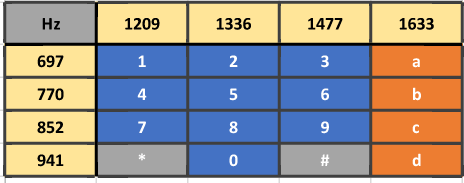
\includegraphics[width=10cm,height=10cm,keepaspectratio]{pictures/DTMF.png}
	\caption{DTMF toner}
	\label{fig:dtmf}
\end{figure}
\newline
Hos DTMF er det vigtigt at hver tone afspilles i længere end 40 millisekunde,r og at mellem hver tone er det en pause på 50 millisekunder.

\subsubsection{C++ og SFML}
C++ har pr. standard ikke funktioner til at afspille og optage lyd. Derfor blev biblioteket SFML installeret til at håndtere disse funktioner. SFML er en simple interface til de forskellige komponenter på ens pc, for at lette udviklingen af f.eks. spil og multimedia applikationer.
\newline
De klasser der bliver brugt fra SFML er:
\begin{itemize}
	\item \texttt{sf::Sound}
	\newline Bruges til at afspille lyd.
	
	\item \texttt{sf::\textcolor{dkgreen}{SoundBuffer}}
	\newline Lagring af audio samples der definere en lyd.
	
	\item \texttt{sf::\textcolor{dkgreen}{SoundRecorder}}
	\newline En abstrakt grund klasse til at optage lyd.
	
	\item \texttt{sf::\textcolor{dkgreen}{SoundBufferRecorder}}
	\newline En specialiseret \texttt{SoundRecorder}, der gemmer optaget lyd i en lyd buffer. 
\end{itemize}

\subsubsection{Optag}
Den første problemstilling projektet stødte på i forhold til optag, var at være i stand til at optage en DTMF tone og analysere optagelsen, hvorefter at fortælle hvilken tone der blev optaget.
\\
\newline
Før en optagelse kan finde sted, blev en samplingsfrekvens for optagelse nødvendigvis defineret og fastsat. Denne samplingfrekvens er yderst vigtig for projektet, eftersom denne samplingsfrekvens dikterer hvordan resten af det fysiske lag skal oprettes. 
\newline
Som et krav skal samplingsfrekvensen overholde Nyquist raten:
$$f_s > 2 \times f_{max}$$
\newline
Den højeste frekvens hos en DTMF tone er 1633 Hz, derfor skal samplingsfrekvensen som minimum være 3267 Hz. Til projektet blev samplingsfrekvensen sat til 8000 Hz, eftersom det er en ofte brugt samplingsfrekvens ved implementering af DTMF genkendelse, og at den opretholder Nyquist raten.
\\
\newline
Projektets optagefunktioner hviler tungt på SFML bibliotekets klasser, \texttt{sf::\textcolor{dkgreen}{SoundRecorder}} og \texttt{sf::\textcolor{dkgreen}{SoundBufferRecorder}}, eftersom C++ egets bibliotek ikke tilbyder optagefunktioner.
\\
\newline
Projektets første løsning på at optage en DTMF tone og analysere optagelsen var en simpel løsning, der dog viste sig ikke at være tilstrækkelig for dette projekt.
\newline
En optagelse blev oprettet ved først at lave et objekt f.eks. \texttt{sf::\textcolor{dkgreen}{SoundRecorder}} optag.
\newline
Derefter startede SFML sin egen tråd og optog, når man brugte funktionen \texttt{optag.start(8000)} (8000 Hz for projektets samplingsfrekvens). Koden sættes til at sove den tid der skal optages, hvorefter at optagelsen stoppes med \texttt{optag.stop()}. Optagelsens information blev derefter hentet ved at lave en reference til optagelsens buffer \texttt{sf::\textcolor{dkgreen}{SoundBuffer} \&enBuffer}, derefter blev der oprettet en vektor af pointerer til bufferen \texttt{sf::\textcolor{dkgreen}{Int16*} samples = enBuffer.getSamples();}. Vektoren består nu af diskrete værdier for en optagelse, hvorpå der blev udført en DFT. Denne DFT vil således være i stand til at vise om en DTMF tone er til stede.
\newline
Første løsning på at optage en DTMF tone og analysere optagelsen er ikke forkert, den skabte umiddelbart noget kompleksitet, som projektet blev nødt til at tage højde for:
\begin{itemize}
	\item Løsningen kræver at optageren skal vide hvornår en afspiller af en sekvens af toner er færdig, eftersom analysen af optagelsen først kan finde sted efter en endt optagelse.
	
	\item DFT er en tung udregning. Den har et forhold der siger der er $N^2$ udregninger ved en DFT på N samples. Dvs. efter en optagelse på 10 sekunder sker der
	$$(10 sek \times 8000 Hz)^2 = 6.400.000.000$$
	udregninger, hvilket er en uheldig eksponentiel stigning for udregninger af længere optagelser.
\end{itemize}
Der blev derfor skrevet en klasse \texttt{MyRecorder.h} som arver funktionalitet fra \texttt{sf::\textcolor{dkgreen}{SoundRecorder}} klassen. Der arves 3 funktioner herfra:
\begin{itemize}
	\item \texttt{\textcolor{blue}{virtual bool} onStart()}
	
	\item \texttt{\textcolor{blue}{virtual bool} onProcessSamples(\textcolor{blue}{const} sf::\textcolor{dkgreen}{Int16*}samples, std::\textcolor{dkgreen}{size\_t} sampleCount);}
	
	\item \texttt{\textcolor{blue}{virtual void} onStop();}
\end{itemize}
\texttt{onStart()} og \texttt{onStop()} bliver kørt når et optagelses objekt af \texttt{MyRecorder.h} klassen f.eks. \texttt{\textcolor{blue}{MyRecorder} optag}, bliver startet med \texttt{optag.start()} eller sluttet med \texttt{optag.slut()}. Der kan så defineres start eller slut betingelser for en optagelse, såsom variable eller buffere der cleares.
\newline
\texttt{onProcessSamples()} er en funktion der bliver kørt automatisk og gentaget i samme tråd som optagelsen, afhængigt af hvad for et interval der sættes under \texttt{onStart();} (100 millisekunder pr. standard). Den bliver indlæst med parameteren \texttt{\textcolor{blue}{const} sf::\textcolor{dkgreen}{Int16*} samples}, dvs. en vektor med diskrete værdier for en optagelse, og hver gang funktionen kaldes er det de seneste nye værdier der ligger i vektoren. \texttt{onProcessSamples()} fortsættes med at blive kaldt hvis den returnerer true, og den stoppes hvis der returneres false.
\newline
Dvs. \texttt{MyRecorder.h} klassen kan optage og analysere data på én gang, hvilket løser problematikken om hvorvidt optageren skal vide hvornår den skal optage og afslutte en optagelse. Nu kan der f.eks. laves en starttone og en sluttone, som optageren kan opfange og derfra igangsætte bestemte kode dele.
\newline

Derudover blev klassen \texttt{Goertzel.h} skrevet som alternativ til en DFT udregning.
\newline
\texttt{Goertzel.h} klassen, som navnet antyder, benytter en Goertzel algoritme til at analysere vektoren med de diskrete værdier fra optagelsen. Jf. teori afsnittet, er Goertzel en smart måde hvorpå der kun udføres udregninger på de frekvens bins der ledes efter.
\newline
Dvs. at denne algoritme udfører langt færre udregninger i forhold til DFT og FFT(Fast Fourier Transform), netop fordi der ikke analyseres over alle samtlige DFT/FFT koefficienter. Dette gør at det ikke er noget problem at optage i længere.  
\hfill \break

Før Goertzel algoritmen kan implementeres er der nogle få ting der skal på plads først. Frekvens binsene skal regnes ud, jf. teori om frekvens bins, skal en samplingfrekvens vides og hvor mange samples der skal samples over. Samplingsfrekvensen er fastsat til 8000 Hz, dog skal det antal samples N som Goertzel analyserer over fastsættes. Der er dog nogle pointer ved fastsættelsen af N, jo større N bliver, desto større antal samples skal der udregnes over, men samtidig jo størrer N bliver, jo smallere bliver bredden af frekvens binen, dvs. at den bliver mere præcis. Det handler om at vælge en N, der ikke er for høj, da dette resulterer i tab af beregningshastighed, eller for lav, hvilket resulterer i tab af præcision.
\newline
Derudover må N ikke blive større end 400 samples, jf. teori om DTMF, da der er et tidsrum af 50 millisekunder mellem hver tone, grundet samplingsfrekvensen på 8000 Hz. Dette tidsrum er der for at forhindre, at en analyse af N samples fra en optagelse ikke foregår over et skift fra én tone til en anden.
\newline
Dette taget i betragtning blev N valgt til at være lig 300, eftersom det er tilpas højt for en tilfredsstillende bredde af frekvens binen (8000 Hz / 300 = 26,7 Hz, den må være helt op til 70 Hz før det skaber problemer), samtidig med det tidsrum som projektet faktisk har tilføjet mellem hver tone, kun er på 400 samples, dvs. 50 millisekunder.
\newline
Frekvens binen for hver DTMF frekvens er derfor udregnet, se tabel \ref{fig:tabel}, og kan bruges til implementeringen af \texttt{Goertzel.h} klassen.
\begin{figure}[ht]
	\centering
	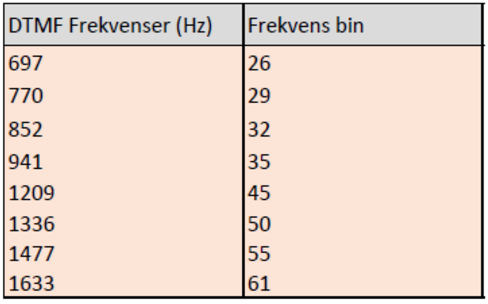
\includegraphics[width=10cm,height=10cm,keepaspectratio]{pictures/DTMFtabel.png}
	\caption{DTMF tabel}
	\label{fig:tabel}
\end{figure}

\subsection{Implementering}
Jf. teori om Goertzel vil filterets G(Z) realiserings struktur se således ud se figur \ref{fig:grs}. Denne realiserings struktur er blevet implementeret i \texttt{Goertzel} klassen ved hjælp af en for løkke, som kører en vektor af diskrete værdier, x(n), med N samples, igennem strukturens udregninger. Husk at ved $x(0) er s(-1) = s(-2) = 0$.
\begin{figure}[ht]
	\centering
	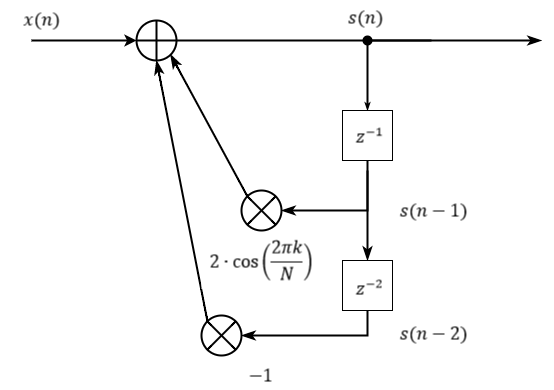
\includegraphics[width=10cm,height=10cm,keepaspectratio]{pictures/GRStruktur.png}
	\caption{Goertzel realiserings struktur}
	\label{fig:grs}
\end{figure} 
\newline
Denne for løkke er blevet implementeret således:
\begin{figure}[ht]
	\centering
	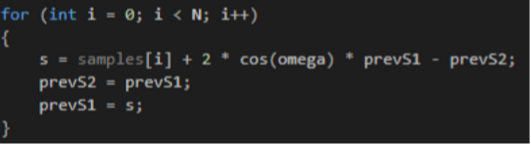
\includegraphics[width=10cm,height=10cm,keepaspectratio]{pictures/Forloop.png}
%	\caption{Goertzel realiserings struktur}
	\label{fig:forloop}
\end{figure} 
\newline
Derefter kan DFT koefficienten bestemmes for en givet frekvens bin k, fordi nu kendes værdierne for sekvensen $s(n)$ ved $s(N-1)$ og $s(N-2)$ (prevS1 og prevS2):
$$|X(k)|^2 = s(N-1)^2 + s(N-2)^2 - 2 \times cos\bigg(\frac{2 \pi k}{N}\bigg) s(N-1)s(N-2)$$
\newline
\texttt{Goertzel} klassens funktion er delt op i 2 metoder:
\begin{itemize}
	\item \texttt{\textcolor{blue}{int} detectFreqs(const sf::\textcolor{dkgreen}{Int16*} samples, \textcolor{blue}{int} K);}
	
	\item \texttt{\textcolor{blue}{int} findTone(const sf::\textcolor{dkgreen}{Int16*} samples);}
\end{itemize}
\texttt{detectFreqs()} bruger det ovenstående implementerede princip, hvorimod \texttt{findTone()} er en metode som bruger \texttt{detectFreqs()} til at gennemgå de tidligere nævnte frekvens bins og returnere en DTMF tone der er over en grænseværdi i forhold til DFT koefficienten. Tonerne er blevet defineret som integers fra 0 til 15, og en grænseværdi er nødvendig fordi en tilfældig støj der rammer en frekvens bin kan blive opfanget.
\newline
\texttt{MyRecorder} har seks metoder:
\begin{itemize}
	\item \texttt{\textcolor{dkgreen}{vector} <\textcolor{blue}{int}> getBesked();}
	
	\item \texttt{\textcolor{blue}{bool} getNyBesked();}
	
	\item \texttt{\textcolor{blue}{bool} getBeskedBegyndt();}
\end{itemize}
\texttt{getBesked()} er den metode der kaldes for at hente de DTMF toner, som blev optaget.
\newline
\texttt{getNyBesked()} og \texttt{getBeskedBegyndt()} er metoder til at kalde boolske udtryk, som bliver brugt til at manipulere og styre \texttt{MyRecorder}.
\begin{itemize}
	\item \texttt{\textcolor{blue}{virtual bool} onStart();}
	
	\item \texttt{\textcolor{blue}{virtual bool} onProcessSamples(\textcolor{blue}{const} sf::\textcolor{dkgreen}{Int16*} samples, std::\textcolor{dkgreen}{size\_t} sampleCount);}
	
	\item \texttt{\textcolor{blue}{virtual bool} onStop();}
\end{itemize}
\texttt{onStart()}, \texttt{onProcessSamples()} og \texttt{onStop()} fungere som tidligere nævnt, dog kaldes \texttt{findTones()} fra \texttt{Goertzel} klassen under hver \texttt{onProcessSamples()} kald, netop fordi der skal optages og analyseres samtidigt.
\hfill \break

For at gøre det nemmere at skrive funktionaliteterne for klasserne \texttt{MyRecorder} og \texttt{Goertzel}, blev der taget udgangspunkt i sekvensdiagrammet SE BILLEDE BILAG WHATEVER. 
\newline
\texttt{MyRecorder} bliver kaldt af \texttt{ToneKonvertering} i det, at det er den klasse som skal modtage beskeden, som består af en vektor af toner, som derefter bliver pullet op igennem applikationens forskellige lag.
\newline
Når \texttt{ToneKonvertering} kalder \texttt{MyRecorder}, blev funktionaliteten for, hvorledes om en optagelse fanger en besked eller ej og om hvor lang en optagelse er, nødt til at blive implementeres under \texttt{ToneKonvertering}s metoden \texttt{returnBitString()}.
\newline
Der er blevet implementeret en while løkke, som kører enten indtil der er gået 10 sekunder, eller at en sluttone på en besked blev opfanget. Der er en if sætning der tester for, om en starttone er blevet hørt, hvis den fanges, skal timeren tælle til 10 forfra. Herefter returneres en vektor med alle de optagede toner. Dvs. at optagelsen altid vil være maks. 10 sekunder lang, hvilket resten af applikationen tager højde for.
\newline
\texttt{MyRecorder} starter en optagelse med samplingsfrekvensen 8000 Hz i dens egen tråd, når metoden \texttt{start(8000)} bliver kaldt. \texttt{onProcessSampling()} kaldes hvert 10’ende millisekund i denne tråd. Under hvert kald bliver de optagede samples analyseret af Goertzel, som returnere tonen for de samples. Denne tone gemmes i \texttt{resusltatVektor}’en, som indeholder de toner, som hele optagelsen opfangede. Udover dette, sker der en mindre sortering af tonerne der optages under \texttt{onProcessSampling()} (dette fremgår ikke af sekvensdiagrammet). Tonerne skal ikke gemmes i \texttt{resusltatVektor}’en medmindre der først har været en starttone. Ved en sluttone stoppes \texttt{onProcessSampling()} for at blive kaldt igen, medmindre en helt ny optagelses session startes. Start og stop tonerne er blevet  defineret som tone 15 (D) = start og tone 14 (\#) = stop. Disse to toner bliver tilført som flag og taget højde for i de øvrige lag.